% Problem 1
\Needspace{18\baselineskip}
\item \label{prob:1}
Two identical mass objects are launched with the same speed from the same starting location. Object 1 is launched at an angle of $30^\circ$ above the horizontal while Object 2 is launched at an angle of $60^\circ$ above the horizontal. Ignore air resistance and consider the flight of each object from launch until it returns to the same launch height above the ground. Which object experiences the greatest change in the linear momentum?
\begin{enumerate}[label=(\Alph*)]
    \item Object 1 since it has a higher final speed.
    \item Object 2 since it has a higher final speed.
    \item Object 2 since it is in the air for a longer time.
    \item The change in momentum is the same for each.
    \item It cannot be determined without more information.
\end{enumerate}

\category{Kinematics \& Momentum}
\StudyGuideLinks{1}
\ProblemSource{1}
\begin{answerbox}
\finalanswer{(C) Object 2 since it is in the air for a longer time.}
\end{answerbox}
\begin{insightbox}
Impulse $J=\int F\,dt=mgT$ (only weight acts). For the same launch speed $v_0$, the time in the air is $T=\tfrac{2v_0\sin\theta}{g}$, so $|\Delta\vec p|=mgT=2mv_0\sin\theta$ increases with $\sin\theta$.
\end{insightbox}
\begin{solutionbox}
Gravity supplies impulse $\Delta\vec p=m\vec gT$. For a return to the launch height, $T=2v_0\sin\theta/g$, so
\[
 |\Delta\vec p|=mgT=2mv_0\sin\theta.
\]
Both objects have the same mass and launch speed, and $\sin60^\circ>\sin30^\circ$. Object 2 therefore has the greater momentum change.
\end{solutionbox}

% Problem 2
\Needspace{18\baselineskip}
\item \label{prob:2}
A mass $m$ is pulled outward until the string of length $L$ to which it is attached makes a 90-degree angle with the vertical. The mass is released from rest and swings through a circular arc. What is the tension in the string when the mass swings through the bottom of the arc?
\begin{enumerate}[label=(\Alph*)]
    \item 0
    \item $mg$
    \item $2mg$
    \item $3mg$
    \item It cannot be determined.
\end{enumerate}

\category{Circular Motion \& Energy}
\StudyGuideLinks{2}
\ProblemSource{2}
\begin{answerbox}
\finalanswer{(D) 3mg}
\end{answerbox}
\begin{insightbox}
Use energy to get $v^2=2gL$ at the bottom, then $T-mg=mv^2/L$.
\end{insightbox}
\begin{solutionbox}
By conservation of energy from the side to the bottom:
\begin{align*}
E_i &= K_i + U_i = 0 + mgL = mgL \\
E_f &= K_f + U_f = \tfrac{1}{2}mv^2 + 0
\end{align*}
Thus $mgL = \tfrac{1}{2}mv^2 \Rightarrow v^2 = 2gL$. At the bottom, radial (inward from the pivot) force balance yields
\[
T - mg = \frac{mv^2}{L} = \frac{m(2gL)}{L} = 2mg \Rightarrow T = 3mg.
\]
\\
\emph{Used:} conservation of mechanical energy and $F_c=mv^2/r$.
\end{solutionbox}

% Problem 3
\Needspace{18\baselineskip}
\item \label{prob:3}
\noindent\begin{minipage}[t]{0.6\linewidth}
\vspace{0pt} % Ensures top alignment
A resonance occurs with a tuning fork and an air column of size 39 cm. The next highest resonance occurs with an air column of 65 cm. What is the frequency of the tuning fork? Assume that the speed of sound is 343 m/s.
\begin{enumerate}[label=(\Alph*)]
    \item 329.8 Hz
    \item 527.7 Hz
    \item 659.6 Hz
    \item 879.5 Hz
    \item 1319 Hz
\end{enumerate}
\end{minipage}%
\hfill
\begin{minipage}[t]{0.33\linewidth}
\vspace{0pt} % Ensures top alignment
\centering
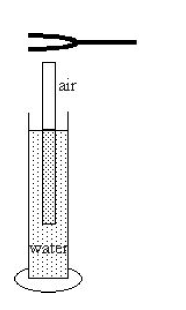
\includegraphics[width=0.7\linewidth]{Problem_03_Figure.png}
\end{minipage}

\category{Waves \& Sound}
\StudyGuideLinks{3}
\ProblemSource{3}
\begin{answerbox}
\finalanswer{(C) 659.6 Hz}
\end{answerbox}
\begin{insightbox}
Closed-tube resonances are spaced by $\lambda/2$; determine $\lambda$ from the difference in lengths and compute $f=v/\lambda$.
\end{insightbox}
\begin{solutionbox}

For a closed tube, successive resonances differ by $\Delta L = \tfrac{\lambda}{2}$. In this case $\Delta L = 0.65\,\text{m} - 0.39\,\text{m} = 0.26\,\text{m}$, so $\lambda = 2\times 0.26 = 0.52\,\text{m}$. The frequency is
\[
 f = \frac{v}{\lambda} = \frac{343\,\text{m/s}}{0.52\,\text{m}} \approx 659.6\,\text{Hz}.
\]
\\
\emph{Model:} closed–open tube has harmonics $L=(2n-1)\lambda/4$, so successive $L$ differ by $\lambda/2$.
\end{solutionbox}

% Problem 4
\Needspace{18\baselineskip}
\item \label{prob:4}
A mass of material exists in its solid form at its melting temperature $10^\circ$C. The following processes then occur to the material:
\begin{itemize}
    \item Process 1: An amount of thermal energy $Q$ is added to the material and $\tfrac{3}{4}$ of the material melts.
    \item Process 2: An identical additional amount of thermal energy $Q$ is added to the material and the material is now a liquid at $50^\circ$C.
\end{itemize}
What is the ratio of the latent heat of fusion to the specific heat of the liquid for this material?
\begin{enumerate}[label=(\Alph*)]
    \item $80^\circ$C
    \item $60^\circ$C
    \item $40^\circ$C
    \item $20^\circ$C
    \item More information is needed to answer this question.
\end{enumerate}

\category{Thermodynamics \& Phase Change}
\StudyGuideLinks{4}
\ProblemSource{4}
\begin{answerbox}
\finalanswer{(A) 80$^{\circ}$C}
\end{answerbox}
\begin{insightbox}
Two equal heat inputs: first melts 3/4, second completes melting 1/4 and warms; equate heats to find $L_f/c_l$.
\end{insightbox}
\begin{solutionbox}

Let mass $m$, latent heat $L_f$, liquid specific heat $c_l$, melting temperature $T_m=10^{\circ}\text{C}$. Process 1: $Q=\tfrac{3}{4}mL_f$. Process 2: $Q=\tfrac{1}{4}mL_f + mc_l(50-10)$. Equate:
\begin{align*}
\tfrac{3}{4} mL_f &= \tfrac{1}{4} mL_f + 40 m c_l \\
\tfrac{1}{2} mL_f &= 40 m c_l \Rightarrow \frac{L_f}{c_l} = 80\,\mathrm K.
\end{align*}
This is a temperature difference of $80^\circ\mathrm C$, corresponding to choice A.
\end{solutionbox}

% Problem 5
\Needspace{18\baselineskip}
\item \label{prob:5}
\noindent\begin{minipage}[t]{0.6\linewidth}
\vspace{0pt}
What is the ideal mechanical advantage for the pulley system shown in the figure?
\begin{enumerate}[label=(\Alph*)]
    \item $F/Mg$
    \item $Mg/F$
    \item 3
    \item 4
    \item 5
\end{enumerate}
\end{minipage}%
\hfill
\begin{minipage}[t]{0.33\linewidth}
\vspace{0pt}
\centering
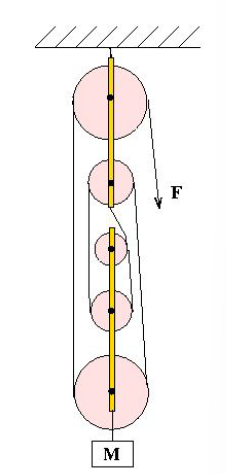
\includegraphics[width=0.6\linewidth]{Problem_05_Figure.png}
\end{minipage}

\category{Simple Machines \& Statics}
\StudyGuideLinks{5}
\ProblemSource{5}
\begin{answerbox}
\finalanswer{(D) 4}
\end{answerbox}
\begin{insightbox}
Ideal mechanical advantage equals the number of load-supporting rope segments: 4.
\end{insightbox}
\begin{solutionbox}

The ideal mechanical advantage equals the number of rope segments supporting the load. Here the movable block is supported by 4 segments, so $\text{IMA}=4$.
\\
\emph{Reminder:} massless, frictionless rope $\Rightarrow$ equal tension in all supporting segments.
\end{solutionbox}

% Problem 6
\Needspace{18\baselineskip}
\item \label{prob:6}
In a calorimeter, 20 grams of liquid water at $100^\circ$C is mixed with 50 grams of water vapor at $100^\circ$C. The system is allowed to come to equilibrium. Assume the phases coexist at their saturation pressure and the calorimeter and surroundings can be ignored. Which choice best describes the net energy exchange between the vapor and liquid?
\begin{enumerate}[label=(\Alph*)]
    \item There is no net energy exchange.
    \item Energy is transferred from the vapor to the liquid, vaporizing some of the liquid.
    \item Energy is transferred from the vapor to the liquid, increasing the liquid’s temperature.
    \item Energy is transferred from the vapor to the liquid until all of the liquid vaporizes.
    \item Energy is transferred from the vapor to the liquid, condensing some of the vapor.
\end{enumerate}

\category{Thermodynamics \& Phase Equilibrium}
\StudyGuideLinks{6}
\ProblemSource{6}
\begin{answerbox}
\finalanswer{(A) There is no net energy exchange.}
\end{answerbox}
\begin{insightbox}
At 100\textcelsius\ both phases are at the same temperature. In an isolated system the mixture stays at 100\textcelsius; any condensation of vapor must be balanced by vaporization of the same mass of liquid, so the net energy transferred between phases is zero.
\end{insightbox}
\begin{solutionbox}

As both steam and water are initially at the saturation temperature 100°C and the container is isolated (no heat to the surroundings), the final temperature is still 100°C. Let a mass $m_c$ of vapor condense (releasing $m_cL_v$) and a mass $m_v$ of liquid evaporate (absorbing $m_vL_v$). Conservation of energy for the constant-temperature closed system requires $m_cL_v=m_vL_v\Rightarrow m_c=m_v$. Therefore, the energy transferred from vapor to liquid equals the energy transferred from liquid to vapor, and the net energy transfer between the two phases is zero.
\end{solutionbox}

% Problem 7
\Needspace{18\baselineskip}
\item \label{prob:7}
\noindent\begin{minipage}[t]{0.6\linewidth}
\vspace{0pt}
For the circuit shown, $\varepsilon = 6.0$ V, $R_1 = 7.0 \Omega$, $R_2 = 3.0 \Omega$, $R_3 = 6.0 \Omega$, and $R_4 = 12.0 \Omega$. After operating for a long time, the circuit reaches steady state (the capacitor branch is effectively open). What is the voltage across the capacitor at steady state?
\begin{enumerate}[label=(\Alph*)]
    \item 6.0 V
    \item 4.2 V
    \item 3.0 V
    \item 2.2 V
    \item 0.2 V
\end{enumerate}
\end{minipage}%
\hfill
\begin{minipage}[t]{0.33\linewidth}
\vspace{0pt}
\centering
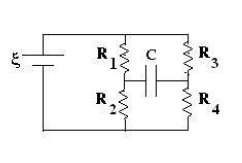
\includegraphics[width=\linewidth]{Problem_07_Figure.png}
\end{minipage}

\category{DC Circuits}
\StudyGuideLinks{7}
\ProblemSource{7}
\begin{answerbox}
\finalanswer{(D) 2.2 V}
\end{answerbox}
\begin{insightbox}
At steady state the capacitor branch is open; find node voltages by dividers and subtract them.
\end{insightbox}
\begin{solutionbox}

After a long time, the capacitor branch is open. Two independent dividers yield $V_A = 6\,\text{V}\cdot\tfrac{3}{7+3} = 1.8\,\text{V}$ and $V_B = 6\,\text{V}\cdot\tfrac{12}{6+12} = 4.0\,\text{V}$. Thus $V_C = |V_B-V_A| = 2.2\,\text{V}$.
\par\smallskip Equivalent node-voltage viewpoint: with the capacitor open, KCL at the top nodes gives the same divider values; the capacitor voltage is the node difference $|V_B-V_A|$.
\end{solutionbox}

% Problem 8
\Needspace{18\baselineskip}
\item \label{prob:8}
\noindent\begin{minipage}[t]{0.55\linewidth}
\vspace{0pt}
An electron moves in the plane of the page through two regions of space along the dotted-line trajectory shown in the figure. There is a uniform electric field in Region I directed into the plane of the page. There is no electric field in Region II. What is a necessary direction of the magnetic field in regions I and II? Ignore gravitational forces.
\begin{enumerate}[label=(\Alph*)]
    \item Region I: Downward along the page, Region II: Upward along the page
    \item Region I: Upward along the page, Region II: Into the page
    \item Region I: Upward along the page, Region II: Out of the page
    \item Region I: Downward along the page, Region II: Out of the page
    \item Region I: Into the page, Region II: Upward along the page
\end{enumerate}
\end{minipage}%
\hfill
\begin{minipage}[t]{0.4\linewidth}
\vspace{0pt}
\centering
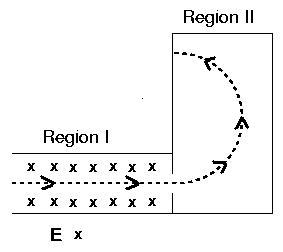
\includegraphics[width=\linewidth]{Problem_08_Figure.png}
\end{minipage}

\category{Electricity \& Magnetism}
\StudyGuideLinks{8}
\ProblemSource{8}
\begin{answerbox}
\finalanswer{(C) Region I: Upward along the page, Region II: Out of the page}
\end{answerbox}
\begin{insightbox}
Use $\vec F_B=q\,\vec v\times\vec B$ and the negative charge of an electron to choose the $\vec B$ directions that curve the trajectory as shown.
\end{insightbox}
\begin{solutionbox}

In Region I, $\vec F_E$ on the electron is out of the page, so $\vec F_B$ must be into the page; with $q<0$, this requires $\vec v\times\vec B$ out of the page, hence $\vec B$ upward along the page. In Region II, curvature upward along the page implies $\vec F_B$ upward along the page. With $q<0$ and $\vec v$ rightward, $\vec B$ is out of the page.
\end{solutionbox}

% Problem 9
\Needspace{18\baselineskip}
\item \label{prob:9}
\noindent\begin{minipage}[t]{0.6\linewidth}
\vspace{0pt}
For the circuit shown, when a shorting wire (no resistance) connects the points labeled A and B, which of the numbered light bulbs become brighter? Assume that all four bulbs are identical and have resistance R.
\begin{enumerate}[label=(\Alph*)]
    \item Bulb 1 only
    \item Bulb 2 only
    \item Bulb 3 only
    \item Bulbs 1 and 3 only
    \item Bulbs 1, 2, and 3
\end{enumerate}
\end{minipage}%
\hfill
\begin{minipage}[t]{0.33\linewidth}
\vspace{0pt}
\centering
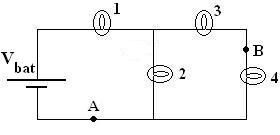
\includegraphics[width=\linewidth]{Problem_09_Figure.png}
\end{minipage}

\category{DC Circuits}
\StudyGuideLinks{9}
\ProblemSource{9} 
\begin{answerbox}
\finalanswer{(D) Bulbs 1 and 3 only}
\end{answerbox}
\begin{insightbox}
Shorting A to B bypasses bulb 4 and changes the currents in the remaining branches.
\end{insightbox}
\begin{solutionbox}

Label the left node at the bottom of the source A and the right mid node B (see figure). Bulbs 1 and 3 are on the top branches left and right of the central vertical branch containing bulb 2; bulb 4 is on the right outer branch.

Let the battery voltage be $V$. Initially bulb 1 is in series with bulb 2 in parallel with bulbs 3 and 4 in series. The equivalent resistance is $R+(R\parallel2R)=5R/3$. Thus $I_1=3V/(5R)$, $I_2=2V/(5R)$, and $I_3=I_4=V/(5R)$.

After A and B are connected, bulb 4 is shorted. Bulb 1 is in series with bulbs 2 and 3 in parallel, giving $R_{\rm eq}=3R/2$. The new currents are $I_1=2V/(3R)$, $I_2=I_3=V/(3R)$, and $I_4=0$. Because $P=I^2R$ for identical bulbs, bulbs 1 and 3 brighten; bulb 2 dims and bulb 4 goes out.
\end{solutionbox}

% Problem 10
\Needspace{18\baselineskip}
\item \label{prob:10}
A car moves to the right along a one-dimensional track for total time $T$ in two parts. Part One: The car maintains constant non-zero speed $V$ for the first $\tfrac{3}{4}$ of the total time. Part Two: The car accelerates uniformly to rest during the last $\tfrac{1}{4}$ of the total time. What is the ratio of the distance traveled during Part One of the trip to the distance traveled during Part Two of the trip?
\begin{enumerate}[label=(\Alph*)]
    \item 6:1
    \item 3:2
    \item The values of V and T are required to answer the question.
    \item 4:3
    \item 8:3
\end{enumerate}

\category{Kinematics}
\StudyGuideLinks{10}
\ProblemSource{10} 
\begin{answerbox}
\finalanswer{(A) 6:1}
\end{answerbox}
\begin{insightbox}
Distance 1: $V\cdot 3T/4$; distance 2: $(V/2)\cdot T/4$. Ratio is 6:1.
\end{insightbox}
\begin{solutionbox}

Part one: $d_1=V\cdot (3T/4)=\tfrac{3}{4}VT$. Part two (uniform decel from $V$ to 0 over $T/4$): $\bar v = V/2$, so $d_2=\bar v\cdot (T/4)=\tfrac{1}{8}VT$. So $d_1:d_2=6:1$.
\end{solutionbox}
